\documentclass[11pt,nocut]{article}

\usepackage{../latex_style/packages}
\usepackage{../latex_style/notations}
%\externaldocument{../lecture_02/lecture_02}
\externaldocument{../lecture_07/lecture_07}


\title{\vspace{-2.0cm}%
	Optimization and Computational Linear Algebra for Data Science\\
Lecture 9: Convex functions}
\author{Léo \textsc{Miolane} \ $\cdot$ \ \texttt{leo.miolane@gmail.com}}
\date{\today}

\begin{document}
\maketitle
\textbf{Warning:}
\emph{This material is not meant to be lecture notes. It only gathers the main concepts and results from the lecture, without any additional explanation, motivation, examples, figures...
}


\section{Convex sets}

\begin{definition}[Convex set]
	A set $C \subset \R^n$ is \emph{convex} if for all $x,y \in C$ and all $\alpha \in [0,1]$,
	$$
	\alpha x + (1-\alpha) y \in C.
	$$
\end{definition}

\begin{figure}[h!]
	\begin{center}
	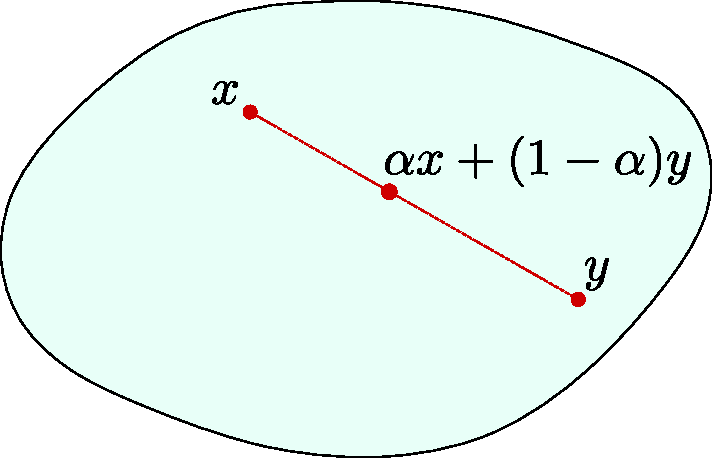
\includegraphics[width=0.4\textwidth]{figures/convex.pdf}
	\hspace{0.9cm}
	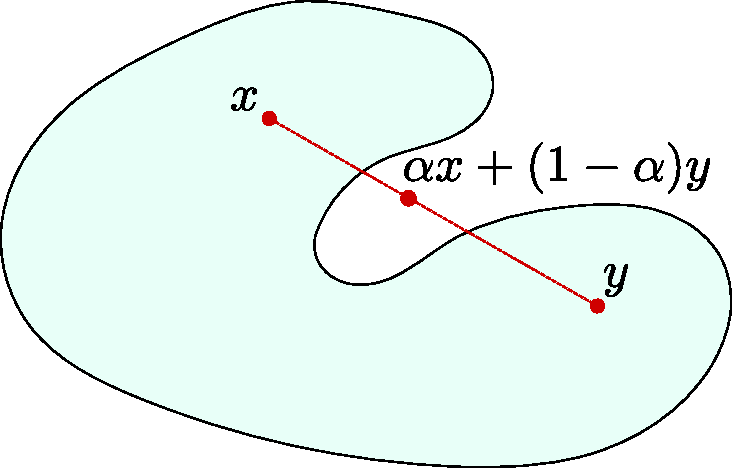
\includegraphics[width=0.4\textwidth]{figures/non_convex.pdf}
	\end{center}
	\caption{Left: a convex set. Right: a non-convex set.}
\end{figure}
\begin{definition}[Convex combination]
	We say that $y \in \R^n$ is a convex combination of $x_1, \dots, x_k \in \R^n$ if there exists $\alpha_1, \dots, \alpha_k \geq 0$ such that
	$$
	y = \sum_{i=1}^k \alpha_i x_i \qquad \text{and} \qquad \sum_{i=1}^k \alpha_i = 1.
	$$
\end{definition}

\begin{proposition}
	If $C$ is convex then all convex combination of elements of $C$ remains in $C$.
\end{proposition}

\section{Convex functions}

\begin{definition}
	A function $f: \R^n \to \R$ is convex if for all $x,y \in \R^n$ and all $\alpha \in [0,1]$,
	\begin{equation}\label{eq:def_convex}
	f(\alpha x + (1-\alpha) y) \leq \alpha f(x) + (1-\alpha) f(y).
\end{equation}
We say that $f$ is \emph{strictly convex} is there is strict inequality in \eqref{eq:def_convex} whenever $x \neq y$ and $\alpha \in (0,1)$.
\\
A function $f$ is concave (respectively strictly concave) if $-f$ is convex (respectively strictly convex).
\end{definition}
\begin{figure}[h!]
	\begin{center}
	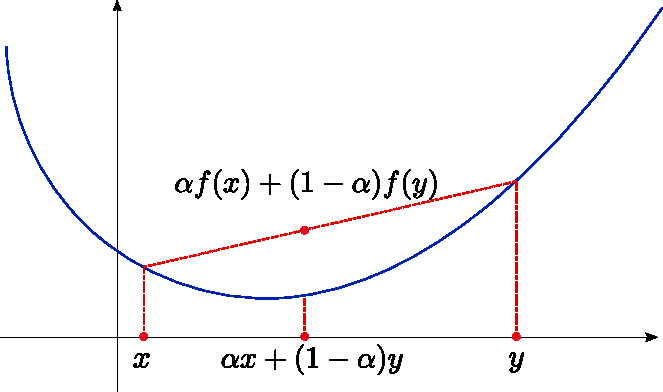
\includegraphics[width=0.7\textwidth]{figures/convex_function.pdf}
	\end{center}
	\caption{A convex function.}
\end{figure}

Notice that a linear function is also a convex function since it verifies \eqref{eq:def_convex} with equality.


\begin{exercise}
	Let $f : \R^n \to \R$ a convex function and $\alpha \in \R$. Show that the ``$\alpha$-sublevel set''
	$$
	C_{\alpha} = \big\{ x \in \R^n \, \big| \, f(x) \leq \alpha \big\}
	$$
	is convex.
\end{exercise}



\subsection{Convex function and differential}

\begin{proposition}
	A differentiable function $f: \R^n \to \R$ is convex if and only if for all $x,y \in \R^n$
	$$
	f(y) \geq f(x) + \nabla f(x)^{\sT} (y-x).
	$$
\end{proposition}

\begin{corollary}
	Let $f: \R^n \to \R$ be a differentiable convex function and $x \in \R^n$. Then
	$$
	x \ \text{is a minimizer of} \ f
	\quad \Longleftrightarrow \quad \nabla f(x) = 0.
	$$
\end{corollary}

\begin{proposition}\label{prop:hessian}
	Let $f: \R^n \to \R$ be a twice-differentiable function. We denote by $H_f$ the Hessian matrix of $f$.
	Then $f$ is convex if and only if for all $x \in \R^n$, $H_f(x)$ is positive semi-definite.
\end{proposition}
When $f: \R \to \R$ is twice differentiable, we get that $f$ is convex if and only if $f'' \geq 0$.

It can be complicated to check that a function $f$ is convex using Proposition \ref{prop:hessian} when $n \geq 2$. The next proposition shows that we can always reduce to the unidimensional case, by checking that the restriction of $f$ on every line is convex:

\begin{proposition}
	A function $f: \R^n \to \R$ is convex if and only if the function
	$$
	\begin{array}{rccc}
		g: & \R & \to & \R \\
		   & t & \mapsto & f(x+t v)
	\end{array}
	$$
	is convex for all $x,v \in \R^n$.
\end{proposition}

\subsection{Jensen's inequality}

\begin{proposition}[Jensen's inequality]\label{prop:jensen}
	Let $f: \R^n \to \R$ be a convex function. Then for all $x_1, \dots, x_k \in \R^n$ and all $\alpha_1, \dots, \alpha_k \geq 0$ such that $\sum_{i=1}^k \alpha_i = 1$ we have
	$$
	f\left(\sum_{i=1}^k \alpha_i x_i \right) \leq \sum_{i=1}^k \alpha_i f(x_i).
	$$
	More generally, if $X$ is a random variable that takes value in $\R^n$ we have
	$$
	f\big(\E [X]\big) \leq \E \big[f(X)\big].
	$$
\end{proposition}
\begin{remark}
	If $f$ is concave then Proposition \ref{prop:jensen} holds, but with inequalities in the reverse order.
\end{remark}

\begin{example}[Discrete entropy]
	Let $Z$ be a random variable that take value in $\{1, \dots, k\}$ and write $p_i = \P(Z = i)$. The entropy of $Z$ is defined as
	$$
	H(Z) = - \sum_{i=1}^k p_i \log(p_i).
	$$
	We apply Jensen's inequality to the concave function $\log$:
	$$
	H(Z) = \sum_{i=1}^k p_i \log(1/p_i) \leq \log\left(\sum_{i=1}^k p_i / p_i\right) = \log(k).
	$$
	Notice that $H(Z) = \log(k)$ when $Z$ is uniformly distributed over $\{1,\dots,k\}$, i.e.\ $\P(Z=i) = 1/k$ for all $i$. \emph{Conclusion}: maximal entropy is achieved for the uniform distribution.
\end{example}


\subsection{Operations that preserve convexity}

\begin{proposition}[Non-negative linear combination of convex functions]
	Let $f_1, \dots, f_k$ be convex functions from $\R^n \to \R$ and let $\alpha_1, \dots, \alpha_k \geq 0$. Then the function $f$ defined by
	$$
	f(x) = \sum_{i=1}^k \alpha_i f_i(x)
	$$
	is convex. In particular a sum of convex functions is convex.
\end{proposition}

\begin{proposition}[Supremum of convex functions]
	Let $(f_i)_{i \in S}$ is a family of convex functions from $\R^n \to \R$. Then the function
	$$
	f(x) = \sup_{i \in S} f_i(x)
	$$
	is convex. In particular, a supremum of affine functions is a convex function.
\end{proposition}

\begin{proposition}[Composition with affine function]
	Let $f: \R^n \to \R$ be a convex function, $A \in \R^{n \times m}$ and $b\in\R^n$.
	Then the function $g: \R^m \to \R$ defined by
	$$
	g(x) = f(Ax + x)
	$$
	is convex.
\end{proposition}


\section*{Further reading}

See \cite{boyd2004convex} Chapters 2 and 3 for example of properties of convex sets/functions. See also \url{http://web.stanford.edu/class/ee364a/lectures.html} for nice lecture slides.
The book \cite{rockafellar1970convex} is a great reference for convex analysis, but is mathematically more involved.


\vspace{1cm}
\centerline{\pgfornament[width=7cm]{71}}


\bibliographystyle{plain}
\bibliography{../references.bib}
\end{document}
